\section{Introduction to \troupelang}
\troupelang\ is a programming language for concurrent and distributed programming with 
dynamic information flow control. 
\troupelang\ is a research language, and as such is intended as a playground for research in 
information flow control.


\subsection{Background and influence}
The design of \troupelang\ is influenced by a number of programming languages and systems. With respect to 
security, our design draws heavily on the systems such as Fabric/Jif, LIO, and FLAM.
With respect to concurrency, the design draws on the systems such as Erlang, Cloud Haskell, and Concurrent ML.
Finally, our syntax is SML-like.





\subsection{Intended audience}
This guide is intended for researchers and graduate-level students\footnote{You have the authors' sympathies if your instructor makes you read this.} interested in \troupelang.
We assume that the reader is familiar with basic functional programming and the 
core concepts of language-based information flow control such as noninterference.


\section{System architecture}
\label{sec:design}
This section describes the basic architecture of the Troupe system
and an overview of the programming model.

\subsection{Troupe architecture}

Two key concepts in Troupe's architecture are \emph{processes} and \emph{nodes}. A process is the primary unit of computation. Processes are lightweight and communicate with each other using message passing. Troupe processes run on Troupe nodes. A node is the primary unit of trust and corresponds to an instance of the Troupe runtime. Each node has a unique network identifier, and all communication between nodes is point-to-point encrypted using standard techniques.


To  enforce information flow control in a decentralized fashion, Troupe combines the notions of standard security levels and \emph{trust} between nodes.
There are no special requirements on the underlying label model other than the standard requirements of the distinguished bottom and top elements, denoted~$\bot$ and~$\top$, operators for the least upper bound and the greatest lower bound, denoted~$\sqcup$ and~$\sqcap$ respectively, and the security ordering $\flowsto$.

Troupe nodes decide for themselves how much they trust other nodes.
Trust is specified via security levels. Every node fully trusts itself, corresponding to trust level~$\top$. Trust levels of selected few nodes are specified through runtime configuration. All other nodes have trust level~$\bot$. Such nodes are assumed to perform no security monitoring on their end. In particular, nodes that do not run Troupe runtime also have trust level~$\bot$ (communication with such nodes is possible for as long as they adhere to the serialization protocol). When communicating with $\bot$-trusted nodes, all data from received them is treated as public (i.e., confidentiality level $\bot$) and no confidential data can be sent to them. 

In general, when node~$n_1$ trusts node~$n_2$ up to level~$\ell$ it means:
\begin{enumerate}
    \item only data labeled up to~$\ell$ is sent from $n_1$ to $n_2$, and 
    \item data received from~$n_2$ by $n_1$ is attenuated to be at most~$\ell$.
\end{enumerate}

\noindent 
The first item prevents sending sensitive information to nodes that are not trusted to protect it. The second item weakens security labels of untrusted nodes.



 We note that trust between nodes may be asymmetric, but is implicitly transitive. Trust should also not be conflated with integrity -- in the current system we only focus on the confidentiality.

Figure~\ref{fig:troupe:architecture} illustrates three Troupe nodes, each running a few processes. The arrows in the figure correspond to the messages between processes. Messages within each node are delivered to processes directly, whereas messages between nodes are subject to inspection by the networking runtime based on the trust levels. % (cf. Section~\ref{sec:io:check}).

\begin{figure}
\begin{center}
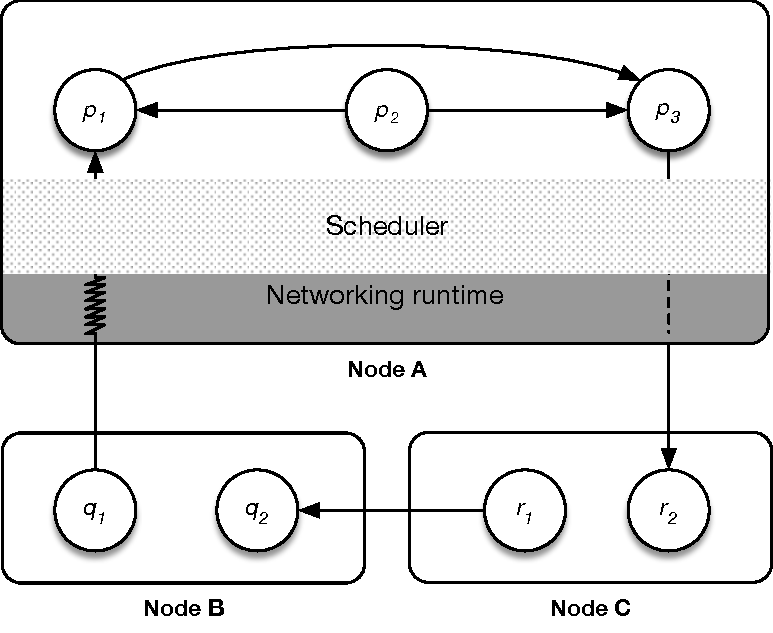
\includegraphics[width=0.5\columnwidth]{process_and_nodes}	
\end{center}
\caption{Nodes and processes in Troupe. The zigzagged line on the incoming message corresponds to message attenuation, the dashed line on the outgoing message corresponds to checking that the recipient is trusted to receive the message.
 \label{fig:troupe:architecture}}
\end{figure}



\subsection{Tag-based label model}
The current version of Troupe uses a simple tag-based label model.
Tags are abstract identifiers, e.g., \tag{alice}, \tag{bob}, \tag{secret},
that specify confidentiality restrictions on data. 
A security level is a set of tags, e.g., 
\lev{\tag{alice}, \tag{bob}}, or 
\lev{\tag{alice, bob, charlie}}.
The more tags there are in the level the more restrictive is the data. 
For example, the level 
\lev{\tag{alice, bob}} is less restrictive than 
\lev{\tag{alice, bob, charlie}}. The least restrictive level is the 
empty set level \lev{}. When two levels are ordered we write 
$\ell_1 \sqsubseteq \ell_2$ to say that level $\ell_2$ is as restrictive 
as $\ell_1$.


%
%{\bf Threat model} 
%Troupe's threat model is one of the \emph{remote attackers} that only observes the messages sent to them or their absence. In particular, the adversary does not observe the state of the Troupe runtime, including local error messages or CPU usage. We also do not address traffic analysis attacks.



\section{Basic features}


\subsection{A minimal \troupelang\ program}


We start with an example of a small \troupelang\ program that returns number 42 as its result.
\begin{verbatim}
42
\end{verbatim}

This program can be compiled, executed, and inspected for the return value using the following sequence of shell commands.
\begin{verbatim}
$ $TROUPE/bin/troupec program.trp -o out.js
$ $TROUPE/rt/troupe out.js --localonly 
...
main thread finished with value: 42@{}%{}
\end{verbatim}

The first command here invokes the \troupelang\ compiler and specifies the generated output file to be {\tt out/program.js}.
The second command invokes the nodejs runtime on the generated file. Note {\tt {-}{-}localonly} flag that 
prevents the runtime from initializing the network layer -- we discuss the network layer in Section~\ref{sec:network}.
Troupe installation also includes a shell script \code{local.sh} that combines the above two tasks of compiling 
and running the programs.

Observe the format of the output value {\tt 42@\{\}\%\{\}}. This value is \emph{labeled} and consists of three 
parts: the base value 42, the security label of the value after the @ sign, 
and the security label of the type after the \% sign. Here,  {\tt \{\}} that means the lowest security level.



\subsection{Overview of the basic language}
At the very core of \troupelang\ is a dynamically typed functional programming language without mutable references. 
For example, a Fibonacci function in \troupelang\ is written exactly as in SML sans type annotations.
\begin{lstlisting}
(* basic_fib.trp *)
let fun fib x = 
        if x > 2 then fib (x - 1) + fib (x - 2)
                 else 1
in fib 10
end
\end{lstlisting}
Running this program results in the output
\begin{verbatim}
main thread finished with value: 55@{}%{}
\end{verbatim}


Note that \troupelang\ is dynamically typed. For example, a program such as {\tt 1 + () } results in a 
runtime type error

\begin{verbatim}
Runtime error in thread b279c491-4509-48e0-82fa-15f18de96003@{}%{}
   value ()@{} is not a number    
\end{verbatim}

\subsection{Types and values}
\troupelang\ has the following types:
\begin{description}
\item [Unit] Unit type with the unit value \textcode{()}.
\item [Booleans] Boolean type with literals \textcode{true} and \textcode{false}.
\item [Number] Number type.
\item [String] String type. String literals are created by placing text between double quotes, e.g., "hello, world".
\item [Tuple] Tuple aggregate, e.g., \textcode{("hello", (), true, 42)}.
\item [List] List aggregate, with empty list denoted as \textcode{[]}.
\item [Function] Function type. Function values are created either using \textcode{fn x => e} syntax or using the let-fun declarations (cf. Sec~\ref{sec:letfun}).
\item [Process Id] Process identifier (cf. Section~\ref{sec:concurrency}).
\item [Label] Security label (cf. Section~\ref{sec:infoflow}).
\item [Authority] Declassification capability (cf. Section~\ref{sec:declassification}).
\end{description}
Note that strings are also used for referring to node identities.


\subsection{Basic operations}
Troupe supports basic arithmetic and comparison operations on numbers. The comparison is also extended to strings. 
Aggregates support equality checks that is defined as point-wise equality of their elements. Boolean conjunction is 
\textcode{andalso}, and boolean disjunction is \textcode{orelse}. List cons operation is \textcode{::} and 
string concatenation is {\textcode{\^{}}}.

\subsection{Thread-local control flow}
Troupe uses SML-like syntax for thread-local operations. A reader familiar
with SML may skip this subsection and proceed to  Section~\ref{sec:labels}.

\subsubsection{If expressions}
Conditionals have the form \textcode{if e0 then e1 else e2}, where \textcode{e0} is the guard of the conditional. 
The branch \textcode{e1} is chosen if \textcode{e0} evaluates to true; otherwise, the branch \textcode{e2} is chosen.

\subsubsection{Case expressions}
Case expressions have the form
\begin{lstlisting}
case e of 
   pat_1 => e_1
 | pat_2 => e_2 
 |  ...
 | pat_n => e_n
\end{lstlisting}
Here, \textcode{pat\_1}, ..., \textcode{pat\_n} are the patterns that are matched against the expression \textcode{e}, and the \textcode{e\_1}, ..., \textcode{e\_n} are the 
expressions to evaluate. Patterns range over literals, including \textcode{()}, booleans, numbers, and string literals, as well as the 
aggregate constructors, and the wildcard pattern \_.



\subsubsection{Let expressions}
Let expressions are used for binding names to values. The basic value binding uses the \textcode{let val} syntax. 
Several binding may appear in one block, and references to the earlier bindings in the block are allowed. 
\begin{lstlisting}
let val x = 20
    val y = x + 2
in x + y
end  
\end{lstlisting}


\subsubsection{Function declarations}
\label{sec:letfun}
Functions are declared using \textcode{let fun} syntax. Mutually recursive functions 
are delimited using the \textcode{and} keyword.
\begin{lstlisting}
(* basic_evenodd.trp *)
let fun even x = if x = 0 then true else odd (x - 1)
    and odd x = if x = 0 then false else even (x - 1)
in even 7
end    
\end{lstlisting}

Function application has the form \textcode{e0 e1}. Curried function declarations and partial 
application is supported, e.g.:
\begin{lstlisting}
let fun add2 x y = x + y 
    val inc = add2 1 
in inc 10
end    
\end{lstlisting}



\subsection{Libraries}
\label{sec:labels}
Troupe has a minimal support for built-in libraries. Current libraries include a library \code{lists} for common list manipulations, library  \code{declassifyutil} for declassification of aggregate data structures, and library
\code{stdio} with convenient wrappers for standard input and output. To use a library, one needs to import it with an \code{import} statement at the top of the program.
\begin{lstlisting}
(* basic_lib.trp *)
import lists 
printWithLabels (map ( fn i => i + 1) [1,2,3])
\end{lstlisting}



\subsection{Concurrency} 
\label{sec:concurrency}
\subsubsection{Spawning processes}
New processes are created using \code{spawn} function that takes as its argument a unit-argument function. 
It return the process identifier of the new process, and starts the new process that from now on runs concurrently with the 
parent process.
\begin{lstlisting}
(* basic_spawn.trp *)
import lists
let fun printwait x = let val _ = printWithLabels x in sleep 10 end
    fun foo () = map printwait [1,2,3]
    fun bar () = map printwait ["A", "B", "C"]
in  (spawn foo, spawn bar)
end
\end{lstlisting}
Execution of this program yields the following output:
\begin{verbatim}
main thread finished with value: (ae07ebcc-8a36-401e-b755-ff2393588c87@{}%{}, 
ed165a5d-acb0-4c6e-9843-29d9f263c6da@{}%{})@{}%{}
1@{}%{}
"A"@{}%{}
2@{}%{}
"B"@{}%{}
3@{}%{}
"C"@{}%{}
\end{verbatim}

\subsubsection{Sending and receiving messages}
Process communication in Troupe happens via message passing.  Every process has a designated mailbox,
and other processes may send messages to that mailbox. Only the process that owns the mailbox may pick the messages from it.


To send a message to another process, we use function \code{send} that accepts as its argument a tuple of
a process identifier and a value to send. To receive a message from the mailbox, we use function \code{receive}
that accepts as its argument a list of handlers that select a message from the mailbox.



\begin{lstlisting}
(* basic_receive.trp *)
let fun foo () =
      receive [hn x => printWithLabels ("foo received", x)]
    val p = spawn foo
in send (p, "hello")
end    
\end{lstlisting}


\paragraph{Handlers}\label{sec:handlers} 
In the example above, the expression \textcode{hn x => ...} is a \emph{handler}. 
Handlers are used for selecting messages from the mailbox. The syntax for handlers is
\begin{center}
 \textcode{hn $\mathit{pat}$ when $\mathit{e_1}$ => $\mathit{e_2}$}
 \end{center}
 
 Here, $\mathit{pat}$ is the pattern to match, $\mathit{e_1}$ is the guard expression, and $\mathit{e_2}$ is the body of the handler. 
 The guard part of the handler (\textcode{when $\mathit{e_1}$)} may be omitted. 
 %
 When several handlers are provided they are used in the order they appear in the list.
Finally, note that, on each invocation of \textcode{receive}, only one message is selected. Subsequent selection
requires another call to \textcode{receive}.
 %
Finally, note that handlers are first class (see also the implementation note below).  

\paragraph{Constraints on the guard expressions}
Evaluation of pattern and guard expressions is \emph{sandboxed} -- it may not invoke I/O operations, or 
spawn threads.


\paragraph{Implementation note} 
Internally, handlers are desugared into a function with a case expression that returns a tuple such that the first 
element of the tuple indicates whether the message should be picked or not, and the second element is the body 
of the handler wrapped in a function, e.g., a value of the form \textcode{fn () => $\mathit{e_2}$}.


\subsubsection{Example: receive with a timeout}
The following listing illustrates a program that implements
receive with a timeout. In the code below, the primitive \textcode{sleep}
suspends the execution of the thread for the specified number of milliseconds,
while the primitive \textcode{mkuuid} creates a unique string.
The use of the unique string avoids creating a confusion when multiple
timeouts may be involved.
\begin{lstlisting}
(* basic_timeout.trp *)
let fun timeout p r t = let val _ = sleep t
                        in send (p, r)
                        end
    val p = self () 
    val r = mkuuid () 
    val _ = spawn ( fn () => timeout p r 1000)    
in receive [ hn ("MESSAGE", x) => print x
           , hn s when s = r => print "timeout" 
           ]
end	
\end{lstlisting}

\subsubsection{Example: updateable service}
The listing below presents an example of an updateable service -- 
this is implemented by having a dedicated handler selecting on 
messages with the \textcode{"UPDATE"} string.

\begin{lstlisting}
(* basic_updateableserver.trp *)
import timeout
let fun v_one n =
         receive [ hn ("REQUEST", senderid) => 
                        let val _ = send (senderid, n) 
                        in v_one (n+1) 
                        end
                 , hn ("UPDATE", newversion) => newversion n
                 ]
                 
    val service = spawn (fn () => v_one 0)
    val _ = send (service, ("REQUEST", self()))
    val _ = receive [ hn x => print x]
                    
    fun v_two n =
        receive [ hn ("REQUEST", senderid) => 
                        let val _ = send (senderid, n) 
                         in v_two (n+1) 
                        end
                , hn ("COMPUTE", senderid, f, x) =>
                        let val _ = send (senderid, f x)
                         in v_two (n+1)
                        end
                , hn ("UPDATE", newversion) => newversion n
                ]

    val _ = send (service, ("UPDATE", v_two))
    val _ = send (service, ("COMPUTE", self(), fn x => x * x, 42))
    val _ = receive [ hn x => print x]
in exitAfterTimeout authority 1000 0 
		"force terminating the server example after 1s"
end    
\end{lstlisting}
The evaluation of this program results in the output
\begin{verbatim}
0@{}%{}
1764@{}%{}
main thread finished with value: ()@{}%{}
force terminating the server example after 1s
\end{verbatim}

\subsection{Debugging concurrent programs}
To help debugging concurrent programs, one can use a special primitive $\code{\_setProcessDebuggingName}$ that
takes a string argument and uses that string when reporting errors in the process. By design, there is no mechanism
for reading the process name other than causing an error; this prevents using process names to leak information.

\section{Information flow control}
\label{sec:infoflow}

This section presents the inner workings of Troupe's security monitor. The monitor is fail-stop at the granularity of individual processes: monitor violation in a process terminates that process but does not affect other processes or nodes.


The monitor is designed to enforce a variant of progress-sen\-si\-tive 
noninterference with declassification. Progress-sensitive baseline is chosen because Troupe is a concurrent system that runs untrusted code, making it possible to amplify leaks via progress/termination, e.g., by designating a process per bit. 
%
In a dynamic system, such as Troupe, a progress leak may stem from several sources that includes divergence, blocking on input, or a runtime crash, such as evaluating the term {\tt 1 + ()}. 
%
%Troupe implements dynamic information flow control. 
%
All information flow violations result in termination of a process,
unless the process is sandboxed. 





\subsection{Privileged operations and authority}
\label{sec:infoflow:authority}

Troupe provides a set of privileged operations 
such as declassifications or process registration. All privileged operations require special \emph{authority} values. 

Authorities in Troupe are capabilities and are unforgeable. 
%They are modeled after similar concepts in Jif~\cite{Jif} and Fabric~\cite{liu2017fabric}, LIO~\cite{LIO} (where they are known as privileges), and operating systems~\cite{HiStar,Asbestos,Flume}.
Operationally, authority is an encapsulated security level that we dub  \emph{efficacy} of an authority\footnote{In standard nomenclature this is simply ``authority level''. However, because authorities in Troupe are values with the corresponding value and type levels, we use a different term to avoid confusion.}. The higher the efficacy level the more powerful is the authority. 
%
System-wide privileged primitives, such as \textcode{register} in the echo-server example require the top authority, while  declassification operations may use attenuated authority. Attenuation happens in one of the following two ways. 
\label{sec:io:check}

\begin{enumerate}
\item 
Programmatic attenuation takes place via a dedicated primitive \textcode{attenuate}. For example, expression \textcode{attenuate( authority, \lev{\ltag{alice}})} returns authority value with efficacy \ltag{\lev{alice}}.  Programmatic attenuation helps programmers apply the principle of least privilege, for example, when passing authority to untrusted code that is allowed to perform some (but not all) declassifications.

\item Troupe runtime attenuates all levels and authority efficacies in remotely received data from $\ell$ to $\ell \sqcap \ell_{\mathit{trust}}$, where~$\ell_{\mathit{trust}}$ is the trust level of the sending node.
\end{enumerate}




In the beginning of program execution, Troupe runtime binds the top authority to the variable \textcode{authority} in the main program. This variable, however, is not in the scope of the code imported from libraries or received over the network. Such code needs to obtain authority explicitly. 




%
%\paragraph{Remark}
%Current version of Troupe only enforces confidentiality 
%properties.
%
%
\subsection{Monitoring for information flow}



\paragraph{Labeled values}
Every value in Troupe is \emph{deeply labeled} with confidentiality
levels. The security level of 
a value specifies the confidentiality policy of the 
value. Troupe uses the syntax \textcode{$\mathit{v}$@\lev{$\mathit{\ell_{\mathit{val}}}$}\%\lev{$\mathit{\ell_{\mathit{type}}}$}} to 
denote that the value $\mathit{v}$ has security level 
$\mathit{\ell_{\mathit{val}}}$, and the information about the type of this value is labeled at $\mathit{\ell_{\mathit{type}}}$.

A labeled value can be created using Troupe's \textcode{raisedTo}
primitive. Troupe's runtime propagates labels throughout the computation.
This section presents examples of label propagation via explicit flows, implicit flows, and
finally via termination and blocking.


\paragraph{Explicit flows}
The following example shows how to create labeled values and how explicit dependencies are propagated.
\begin{lstlisting}
(* ifc_explicit.trp *)
let val x = 10 raisedTo {alice}
    val y = 20 raisedTo {bob}
in x + y
end
\end{lstlisting}
\begin{verbatim}
main thread finished with value: 30@{alice,bob}%{}
\end{verbatim}



\paragraph{Relationship between type and value labels}
Observe how the result of this computation is labeled with 
the level \lev{\tag{alice, bob}}, but the type label is \lev{}.
Because information about the value is more precise than the information about the type, it holds that 
$\ell_{\mathit{type}} \sqsubseteq \ell_{\mathit{val}}$. 



\paragraph{Labels as values and label comparison}
Labels in \troupelang\ are first-class:

\begin{lstlisting}
(* ifc_labels.trp *)
import lists
map (fn (x,lev) => x raisedTo lev) [ (1, {alice})
                                   , (2, {bob})
                                   , (3, {charlie}) ]
\end{lstlisting}
\begin{lstlisting}
>>> Main thread finished with value: [1@{alice}%{}, 2@{bob}%{}, 
3@{charlie}%{}]@{}%{}    
\end{lstlisting}
\paragraph{Implicit flows}
Conditionals propagate the flows as well:


\begin{lstlisting}
(* ifc_implicit1.trp *)
let val x = 10 raisedTo {alice} 
in if x > 5 then 1 else 0 
end	
\end{lstlisting}
\begin{verbatim}
main thread finished with value: 1@{alice}%{alice}	
\end{verbatim}
Observe how the final value carries the dependency of the 
branch that has been chosen here. Because, of the dynamic nature of type checking,
we also carry the information about the chosen branch into the type label.




\paragraph{Implicit flows and I/O}
The implicit information flows are further propagated between processes. 
In the mailbox, each message is additionally tagged with a label that 
corresponds to the blocking level of the sender at the time when the message was sent.
Troupe supports filtering messages based on these tags.
In the following example, \code{rcvp} is a form of receive statement that selects messages
where the pc-tag set to the provided label argument.

\begin{lstlisting}
(* ifc_implicit2.trp *)
let val x = 10 raisedTo {secret}
    val p = self()
    val _ = spawn ( fn () => if x > 0 
    							then send (p, 1) 
    							else send (p, 0) )
in rcvp ({secret}, [ hn x => x ])
end
\end{lstlisting}
\begin{verbatim}
main thread finished with value: 1@{secret}%{secret}
\end{verbatim}


\paragraph{Termination and blocking flows} 
In addition to tracking implicit flows via control flow, Troupe also 
tracks possible leaks via program termination or blocking.
The sources of blocking are all synchronous operations such as receive statements or reading from standard input. 
Each thread has two runtime labels: the program counter label $\mathit{pc}$, and 
the blocking (termination) label $\mathit{block}$. It is always the case that 
$\mathit{pc}~\sqsubseteq~\mathit{block}$. To view the labels there is a 
helper internal function \code{debugpc ()}.
\begin{lstlisting}
(* ifc_debugpc.trp *)
let val x = 1 raisedTo{secret}
    val _ = debugpc() 
    val x = if x > 2 then receive [] else () 
    val _ = debugpc() 
in () 
end    
\end{lstlisting}

Each call to \code{debugpc} prints out the information about the process identifier,
the pc label, and the blocking label.
\begin{verbatim}
PID:2dfe86ae-6bf3-4bfc-8a0c-200230e0296c@{}%{}     PC:{}       BL:{}                
PID:2dfe86ae-6bf3-4bfc-8a0c-200230e0296c@{}%{}     PC:{}       BL:{secret}           
\end{verbatim}
As one can see from the output above, the pc label after the conditional
statement is lowered back to \lev{}, but the blocking label remains tainted 
with the label of the branch. The distinction between the two labels
is helpful when declassifying the blocking label (cf. Section~\ref{sec:pinidecl}).



\paragraph{Implicit flows and type labels}
Type labels of values created in branches are also tainted by the pc-label.
Operations that check the type label, e.g., arithmetics or pattern
matching, use the information in the type label to appropriately taint the blocking level.
the value.
\begin{lstlisting}
(* ifc_type_labels.trp *)
let val x = 100 raisedTo {alice}
    val y = 200 raisedTo {bob}
    val z = 300 raisedTo {charlie}
    val a = let pini authority 
                val a = if y > 10 then z else "not an integer"
            in a 
            end
    val _ = printWithLabels a
    val _ = debugpc()
    val w = a + x
    val _ = printWithLabels w
in debugpc()
end
\end{lstlisting}
\begin{verbatim}
300@{charlie,bob}%{bob}
PID:2dfdc81f-1027-40e2-810c-11fadb2dd40f@{}%{}     PC:{}          BL:{}
400@{charlie,bob,alice}%{}
PID:2dfdc81f-1027-40e2-810c-11fadb2dd40f@{}%{}     PC:{}          BL:{bob}
\end{verbatim}


\paragraph{Implementation note}
\troupelang\ implements information flow enforcement via inlining.



\subsection{Declassification and progress-sensitivity}
\label{sec:declassification}
To relax the constraints imposed by the information flow control, Troupe offers 
a mechanism for \emph{declassification}. 
%\subsubsection{Authority}

In Troupe, declassifying information requires a capability to declassify,
known as the \emph{declassification authority}. 
The authority carries a security level that is the upper bound 
on what information it can declassify. 
%
Given  a value at 
level~$\ell_{\mathit{from}}$, an authority of 
level $\ell_{\mathit{auth}}$ permits a declassification to level 
$\ell_{\mathit{to}}$ if
${\ell_{\mathit{from}}} \sqsubseteq {  \ell_{\mathit{to}} \sqcup \ell_{\mathit{auth}}}.$

%Authorities in Troupe are capabilities, which means that they cannot be 
%created out of thin air. At the start of a Troupe program, the top-level authority is 
% bound to variable \textcode{authority}. This authority can be used freely by the program.
%Note, however, that the authority is not available to code that is imported 
%from the libraries or to code that is received over the network (cf. Section~\ref{sec:network}).


\subsubsection{Example with attenuation of authority}
Authority can be attenuated using the \code{attenuate} primitive. 

\begin{lstlisting}
(* ifc_attenuate.trp *)
attenuate (authority, {alice})    
\end{lstlisting}
\begin{verbatim}
>>> Main thread finished with value: !{alice}@{}%{}    
\end{verbatim}

\subsubsection{Basic declassification}
Troupe provides an explicit declassification command \code{declassify} that takes three arguments: 
the expression to declassify, the authority, and the target label. For example, a basic declassification
looks like this. 
\begin{lstlisting}
(* ifc_declassify_atten.trp *)
let val x = 10 raisedTo {alice}
 in declassify (x , authority, {} )
end 
\end{lstlisting}

When authority for declassification is not sufficient, Troupe returns an error message.
\begin{lstlisting}
(* ifc_declassify_err.trp *)
let val authAlice = attenuate (authority, {alice})
    val x = 1 raisedTo {bob}
in declassify (x, authAlice, {})
end     
\end{lstlisting}

\begin{lstlisting}
Runtime error in thread b469cbef-16d3-4fe8-ac1e-bd21c7e8950d@{}%{}
>> Not enough authority for declassification
 | level of the data: {bob}
 | level of the authority: {alice}
 | target level of the declassification: {}    
\end{lstlisting}

\subsubsection{Declassification of the blocking level}
\label{sec:pinidecl}
The treatment of the blocking and termination labels is often restrictive in practice. To relax this, 
Troupe provides declassification of the blocking label. This is done using 
a variant of the \code{let} declaration that is called \code{let\ pini}. 
This statement requires the authority argument to declassify the blocking label 
after the sequence of the declarations (i.e., just before the \code{in} block).
These declarations are accessible in the body of the let statement at permissive
levels.

\begin{lstlisting}
(* ifc_pini.trp *)
let val x = 10 raisedTo {alice}
    val y = 0
    val z = 
        let pini authority
          val _ = if x > 1000 then receive [] else ()
          val z = y + 1
          val _ = debugpc () 
        in z
        end
    val _ = debugpc()
in z
end
\end{lstlisting}

\begin{verbatim}
PID:54bd148b-912e-4ae9-9787-aaf1166e9bc9@{}%{}     PC:{}       BL:{alice}           
PID:54bd148b-912e-4ae9-9787-aaf1166e9bc9@{}%{}     PC:{}       BL:{}            
>>> Main thread finished with value: 1@{}%{}
\end{verbatim}
Observe that in the above program, the level of the final value \code{z}
is not tainted by the blocking label of the high conditional. 


\paragraph{Implementation note}
The expression \code{let\ pini\ e0} $\mathit{decs}\ $\code{in\ e1\ end } is desugared by the compiler frontend into the form 
\begin{lstlisting}
let val tmp = pinipush e0 
    $\mathit{decls}$
    val _ = pinipop tmp
in e1      
end
\end{lstlisting}
Here, \code{tmp} is a fresh variable that is not part of the user program. Primitives \code{pinipush} and 
\code{pinipop} dynamically scope the part of the execution for which the blocking label is declassified.


\subsection{Information flow control with I/O primitives}
This section may be omitted upon first read as it has a number of information flow subtleties that 
can be omitted when first starting to use the system.
\subsubsection{Generalized receive and mailbox clearances}

I/O operations such as send and receive introduce additional concerns w.r.t. 
information flow control. In particular, because mailbox acts as a mutable state, an extra
care needs to be taken to control information flows through the mailbox structure.


Every message in a mailbox carries an extra label -- the blocking level of the sender. We refer to this 
extra label as the \emph{presence label}.
Receiving a value furthermore propagates the taint of the blocking level from the sender to the receiver via the presence label. 
In order to constrain a receive operation from an accidental raise of the blocking level, Troupe
provides a general receive primitive in the form 
\code{rcv(lev1,lev2,hns)}. Here, \code{lev1} and \code{lev2}
indicate the to and from-levels of the presence labels on the messages, and \code{hns} is the list of 
handlers as before.
The \code{receive} operation we introduced earlier is equivalent to \code{rcvp}
at the level of the current pc label.

While such a form of general receive over an interval of levels is useful, it is also too powerful 
and needs to be further constrained. Consider the following snippet


\begin{lstlisting}
let val _ = if secret then rcv ({}, {alice}, [hn x => x])
                      else ()
in rcv ({}, {}, [hn x => x])
end
\end{lstlisting}

Because the receive in the high branch is on an interval, the value of \code{x} may 
depend on the secret value. In general, one can encode an entire secret in the structure 
of the mailbox. To prevent such programs, Troupe provides a special notion of \emph{mailbox clearance}
that constrains receives on an interval. The mailbox clearance is a proxy for an authority. 
It can be raised using a dedicated command \code{raisembox (lev)} that returns a lowering
capability and lowered with command \code{lowermbox(c, authority)}. 
There are a few constraints related to the mailbox clearance.

\begin{enumerate}
    \item In order to receive on an interval $(\ell_1, \ell_2)$ under $\mathit{pc}$ 
    with mailbox clearance $\ell_{\mathit{clear}}$ it must hold that $\ell_2 \sqcup \mathit{pc} \sqsubseteq \ell_1 \sqcup \ell_{\mathit{clear}}$. 
    This constraint ensures that the mailbox clearance is sufficient for the interval receives. When mailbox clearance is $\bot$ -- as it is in the beginning of the program -- only point intervals of the form $(\ell, \ell)$ where $\mathit{pc} \sqsubseteq \ell$ are allowed.

    \item The $\mathit{pc}$-label of the program point where the mailbox clearance is raised affects the lower bound of the intervals. In particular, if the clearance is raised when the $\mathit{pc}$ counter is $\mathit{pc}_{\mathit{raise}}$, the mailbox structure cannot be influenced by receives that are not as restrictive as $\mathit{pc}_{\mathit{raise}}$; in other words: $ \mathit{pc}_\mathit{raise} \sqsubseteq \mathit{pc} \sqcap \ell_1$, where $\ell_1$ is the lower bound of the interval receive. 
    \item If the process mailbox clearance is raised in a branch, it must be lowered back before reaching the join point of the branch.
\end{enumerate}




\section{Networking}
\label{sec:network}

\subsection{Network identity}
Troupe's runtime connects to a distributed p2p system. 
Each instance of the runtime is associated with a network node that uses a
unique network identifier. The identifier information is typically stored in files,
and is provided as arguments to the runtime at startup.
\begin{verbatim}
$TROUPE/rt/troupe out.js --id=<path_to_id_file>    
\end{verbatim}
If no arguments are provided, the runtime generates a fresh identifier at startup.


\subsubsection{Registering and looking up processes}

Node identifiers can be used to register and look processes up.
Consider a simple echo service:
\label{example:echo}
\begin{lstlisting}
let val _ = register ("echo", self(), authority)
    fun loop () =
        let val _ = receive [ hn ("ECHO", x, sender) 
                                   => send (sender, ("REPLY", x))
                            , hn _ => () ]
        in loop ()
        end
in loop ()
end
\end{lstlisting}
The \code{register} primitive is used to bound a process to a name. Because this is a
system-wide operation, it requires the top authority argument.  If we know 
the node identity and the name at which a process is bound, we can find the process at that node, using the 
\code{whereis} primitive:

\begin{lstlisting}
let val echo = 
        whereis ( "QmNRwNZACPciLS14cZFApwrCcAdbRAXYgztea9m5XwRe4z"
                , "echo")
    val _ = send (echo, ("ECHO", "Hello", self()))
in receive [ hn  x => print x]
end    
\end{lstlisting}

The complete echo example -- including the code above and 
the scripts for generating the identifiers is available at 
\code{\$TROUPE/examples/network/echo}.

\subsubsection{Aliases}
Aliases is a mechanism that allows us to avoid having hardcoded node identifiers in the source code. 
The alias mechanism operates in the way of the traditional Unix hosts files.
To use this mechanism, we need to provide the path to a special alias file that contains a mapping between
alias strings and network identifiers. In the text of the program, an alias string must start with character~"@".


\begin{verbatim}
$TROUPE/rt/troupe out.js --aliases=<path_to_aliases_file>
\end{verbatim}

\subsection{Node trust levels}

By default, all nodes in Troupe are mutually distrusting. This means that 
information sent and received to other nodes is considered to be at level \lev{}.
We can increase trust in certain nodes by 
passing a trust map file that include the identity of the nodes and their maximum
trust level.

    
\subsection{Remote spawning}
If we know of a node identifier, we can spawn a thread on that node. Remote spawning is 
disabled by default, and needs the flag {\verb|--rspawn=true|} to be enabled.
%
To spawn a process on a remote node, the \code{spawn} takes a tuple of arguments,
where the first parameter is the string corresponding to the node identifier of the remote machine.


\subsection{Information flow monitoring and attenuation}
When information at level $\ell_{\mathit{data}}$ is sent to a remote node with trust level 
$\ell_{\mathit{trust}}$, the runtime performs the check
$\ell_{\mathit{data}} \sqsubseteq \ell_{\mathit{trust}}$ to ensure that no sensitive information 
flows to a that can violate confidentiality. Because we have no way of enforcing the 
information flow on the remote node, this also means that 
trust relationship between nodes is transitive.

When receiving information from a remote node at level $\ell_{\mathit{trust}}$, 
data labeled at level $\ell$ receives the actual level $\ell_{\mathit{trust}} \sqcap \ell$. 
This ensures that the runtime is not accidentally tainted by nodes that have low (or none at all) trust.

Authority values that are transferred across the nodes are subject to the same constraints and attenuation.



%\section{Sandboxing}
\clearpage
\appendix
\section{Language reference}

\subsection{Built-in expressions}

\subsubsection{\code{adv}}
\begin{description}
    \item [Description] Simulate sending a value to adversary at level $\{\}$. This function is introduced as a 
    pedagogical convenience as as it removes the necessity to set up a network process when explaining explicit and implicit information flows.
    \item [Arguments] A value to pass to the adversary.
    \item [Returns] Unit.
    \item [Failure behavior] Crashes the current process if the provided value and the blocking label are more restrictive than bottom.
    \item [Example usage] \code{adv\ (42\ raisedTo\ \{alice\})}. 
\end{description}

\subsubsection{\code{attenuate}}
\begin{description}
    \item [Description] Returns the attenuated authority 
    \item [Arguments] A value of authority type.
    \item [Returns] A value of authority type
    \item [Example usage] \code{attenuate ( authority, \{alice\} ) } Note that the above example will generate a runtime error.
\end{description}


\subsubsection{\code{authority}}

\begin{description}
    \item [Description] Return the authority argument implicitly provided to the top-level function of the main program.
The accessibility of this argument follows the standard lexical scoping rules. In particular, expressions received over the network carry over the (potentially attenuated) authority of their originating nodes.
    \item [Arguments] None
\end{description}

\subsubsection{\code{declassify}}
\begin{description}
    \item [Description] Declassifies an expression.
    \item [Arguments] A triple of the form $(\mathit{expr}, \code{authority}, \code{\ell} )$, where $\mathit{expr}$ is the expression to be declassified, $\code{authority}$ is the authority to use for declassification, and \code{\ell} is the target level of declassification.
    \item [Returns] The original value declassified to the target level if there is sufficient authority. 
    \item [Failure behavior] Crashes if the provided authority is insufficient for the declassification.
    \item [Example usage] 
\begin{minipage}[t]{30em}
%\begin{lstlisting}
\begin{verbatim}
let val x = 42 raisedTo {alice}
in print (declassify (x, authority, {})
end    
\end{verbatim}
%\end{lstlisting}


 \end{minipage}

    
\end{description}


\subsubsection{\code{exit}}
\begin{description}
    \item [Description] Exits the Troupe runtime.
    \item [Arguments] A tuple \code{(authority, exitCode)}.
    \item [Returns] Nothing
    \item [Example usage] \textcode{exit(authority, 0)}
\end{description}


\subsubsection{\code{getTime}}
\begin{description}
    \item [Description] Obtains current Unix timestmap
    \item [Arguments] Unit.
    \item [Returns] Number. 
    \item [Example usage] \textcode{getTime()}
\end{description}


\subsubsection{\code{inputLine}}
\begin{description}
\item[Description] Reads a  line from the console.
\item[Arguments] Unit.
\item[Returns] String value.
\item[Blocking behavior] Synchronous. Observe that the blocking label 
is raised to top after this operation, because the user providing the 
input is assumed to operate at level top. To prevent this from happening,
the blocking label can be declassified using the \code{let\ pini} constructs.
See also library functions \code{inputLineWithPini} and \code{inputLineWithPini}
from \code{stdio} library.
\end{description}


\subsubsection{\code{lowermbox}}
\begin{description}
    \item [Description] Lowers the clearance of the current process' mailbox. 
    \item [Arguments] A tuple of the raise capability and authority 
    \item [Returns] Unit. 
    \item [Failure behavior] Fails if the type of the argument is invalid (dynamic type checking). Fails if the authority is insufficient for this lowering, or the provided capability does not match the stack scoping discipline. 
\end{description}


\subsubsection{\code{mkuuid}}
\begin{description}
    \item [Description] Generates a random string.
    \item [Arguments] Unit.
    \item [Returns] A newly generated string.
    \item [Example usage] \textcode{print (mkuuid\ ())}
\end{description}


\subsubsection{\code{node}}
\begin{description}
    \item [Description] Returns node identifier of a process.
    \item [Arguments] Process identifier.
    \item [Returns] String containing a node identifier.
\end{description}




\subsubsection{\code{pinipop}}
\begin{description}
    \item [Description] Pop an authority value from the \emph{pini} stack, and declassify the current blocking level.
    \item [Arguments] A string generated by \code{pinipush}
    \item [Returns] Unit.
    \item [Failure behavior] Crashes if the popped authority is insufficient for the declassification of the blocking level,
or if the provided capability does not match to the last capability generated by the \code{pinipush}.
    \item [Example usage] \textcode{pinipop ()}
\end{description}

\subsubsection{\code{pinipush}}
\begin{description}
    \item [Description] Pushes authority value onto the \emph{pini} stack.
    \item [Arguments] A value of type authority.
    \item [Returns] A string capability to be passed as the argument to \code{pinipop}
    \item [Example usage] \textcode{pinipush (authority)}
\end{description}


\subsubsection{\code{pinipushto}}
\begin{description}
    \item [Description] Pushes authority value onto the \emph{pini} stack,
	 with explicit blocking level. 
    \item [Arguments] A tuple: a value of type authority, and a level.
    \item [Returns] A string capability to be passed as the argument to \code{pinipop}
    \item [Failure behavior] Crashes if the current blocking level does not flow to the level argument.
    \item [Example usage] \textcode{pinipushto (authority, \{bob\})}
\end{description}


\subsubsection{\code{print}}
\begin{description}
    \item [Description] Prints a value on the console omitting its security types.
    \item [Arguments] A value of any type.
    \item [Returns] Unit.
    \item [Example usage] \code{print\ "Hello, world"}
\end{description}


\subsubsection{\code{printWithLabels}}
\begin{description}
    \item [Description] Prints a value on the console including its security types.
    \item [Arguments] A value of any type.
    \item [Returns] Unit.
    \item [Example usage] \code{printWithLabels\ "Hello, world"}
\end{description}


\subsubsection{\code{raiseTrust}}
\begin{description}
    \item [Description] Dynamically raise the trust level of a node.
    \item [Arguments] A triple of a node identifier, root-level authority, and the intended trust level.
    \item [Returns] Unit.
    \item [Failure behavior]. Fails if the argument type is invalid. Fails if the authority argument is not top.
 Fails if the blocking level is not $\bot$.
    \item [Example usage] $\code{raiseTrust("@alicescomputer", authority, \{alice\})}$
\end{description}
Note that the top-level authority is required because this is a privileged operation with system-wide consequences. 




\subsubsection{\code{raisembox}}
\begin{description}
    \item [Description] Raises the clearance of the current process' mailbox. 
    \item [Arguments] A security level
    \item [Returns] A capability for lowering the mailbox level back to the previous value. 
    \item [Failure behavior] Fails if the type of the argument is invalid (dynamic type checking).
\end{description}


\subsubsection{\code{random}}
\begin{description}
    \item [Description] Generates a random number between 0 (inclusive) and 1.
    \item [Arguments] Unit.
    \item [Returns] Number.
    \item [Example usage] \code{random()}
\end{description}





\subsubsection{\code{receive}}
\begin{description}
    \item [Description] Picks a message from the mailbox.
    \item [Arguments] A list of \emph{handler functions} (cf. Section~\ref{sec:handlers}).
    \item [Returns] The value returned by the body of the matching handler.
\end{description}

\subsubsection{\code{register}}
\begin{description}
    \item [Description] Registers the process under a name.
    \item [Arguments] A tuple of the form $(\mathit{str}, \mathit{pid}, \mathit{authority})$, where $\mathit{str}$ is the name under
which the process is to be registered, $\mathit{pid}$ is the process identifier, and 
$\mathit{authority}$ is the top authority value.
    \item [Returns] Unit.
    \item [Blocking behavior] Synchronous. 
    \item [Failure behavior] Crashes if the provided authority is not top, or if the blocking level is not $\bot$.
    \item [Example usage]\textcode{register ("auctionServer", self(), authority)}
\end{description}

Note that this is a privileged operation with system-wide consequences. 


\subsubsection{\code{rcv}}
\begin{description}
    \item [Description] Picks a message from the mailbox with pre-filtering the levels of the messages.
    \item [Arguments] A triple of the form $(\mathit{hs}, \ell_{\mathit{lo}}, \ell_{\mathit{hi}}) $ where $\mathit{hs}$ is the list of handlers, $\ell_{\mathit{lo}}$ is the lower bound on the \emph{sender-level} of the messages, and 
$\ell_{\mathit{hi}}$ is the upper bound on the \emph{sender-level} of the messages in the mailbox.
    \item [Returns] The value returned by the body of the matching handler.
\end{description}


\subsubsection{\code{sandbox}} 
\begin{description}
    \item [Description] Execute a function in a sandbox for a fixed duration of time.
    \item [Arguments] A tuple of the form $(\mathit{t}, f)$, where $t$ is the timeout duration in milliseconds, and $f$ is the function
of the form $\code{fn () => e}$ that is executed in the sandbox. A sandboxed process is heavily restricted: it cannot perform
any I/O operations or spawn new threads. 
    \item [Returns] A tuple of the form $(\mathit{ok}, \mathit{val})$ where $\mathit{ok}$ is either true or false, with true meaning that the sandbox execution has completed successfully, and false meaning that the sandbox has exhibited a crash or timeout. When the evaluation succeeds, value $\mathit{val}$ carries the return value of the sandboxed function; it is a unit value otherwise.
    \item [Blocking behavior] Synchronous. The execution of the process always takes at least duration $\mathit{t}$, even if the sandboxed process successfully finishes before that.
    \item [Failure behavior] This function always succeeds. All internal errors are suppressed.
    \item [Example usage] \textcode{sandbox (1000, fn () => 1 + ()  )}
    \item [Implementation notes] Troupe's current prototype does not yet implement this with high granularity.
\end{description}


\subsubsection{\code{self}}
\begin{description}
    \item [Description] Returns the current process identifier.
    \item [Arguments] Unit.
    \item [Returns] The value of process identifier type.
    \item [Example usage] \textcode{print (self\ ())}
\end{description}


\subsubsection{\code{send}}
\begin{description}
    \item [Description] Sends a message to a process.
    \item [Arguments] A tuple of the form $(\mathit{pid}, v)$ where the $\mathit{pid}$ is the process identifier 
of the recipient process, and $v$ is the value to send.
    \item [Returns] Unit.
    \item [Failure behavior] Crashes the current process if the node hosting the recipient process is untrusted to receive $v$.
This crashing behavior is exhibited only if the process is hosted remotely. Local processes are implicitly fully-trusted because the 
enforcing runtime is the same.
    \item [Blocking behavior] Asynchronous.
\end{description}


\subsubsection{\code{\_setProcessDebuggingName}}
\begin{description}
    \item [Description] Sets the process name that is used in debugging.
    \item [Argument] A string value.
    \item [Returns] Unit.
    \item [Failure behavior] Fails if the type of the argument is invalid (dynamic type checking).
\end{description}



\subsubsection{\code{sleep}}

\begin{description}
    \item [Description] Suspends the execution of the current thread for a specified duration of time.  
    \item [Arguments] One argument of type number that specifies the sleep time in milliseconds.
    \item [Returns] Unit.
    \item [Example usage] \code{sleep\ 100}
\end{description}



\subsubsection{\code{spawn}}
\begin{description}
    \item [Description] Spawns a new process locally or remotely.  
    \item [Arguments] Either a tuple of the form \code{ (nodeid, f )} of a node identifier (as a string) and a function 
or one argument of the type function. 
Note that the function must be of the form \code{fn () => e}, i.e., it must take just one unit argument.
    \item [Returns] The process identifier of the newly spawned process.
    \item [Blocking behavior] Blocks until the new process is created.
    \item [Example usage] \textcode{ print (self (), spawn(fn () => print\ (self()))) }

\end{description}

\subsubsection{\code{raisedTo}}
\begin{description}
    \item [Description] Raises the level of a value. Observe that this expression uses the infix syntax.
    \item [Arguments] An expression of any type and a level.
    \item [Returns] The same expression with its level raised to the provided level.
    \item [Example usage] $\code{42\ raisedTo\ \{alice\}}$
\end{description}


\subsubsection{\code{whereis}}

\begin{description}
    \item [Description] Looks up a registered process on a remote node.
    \item [Arguments] A tuple of the form $(\mathit{nodeid}, \mathit{name})$ where $\mathit{nodeid}$ is the string representing the p2p-identifier of the node, and $\mathit{name}$ is the name of the process registered at that node.
    \item [Returns] The process identifier of the node on the remote machine. 
    \item [Blocking behavior] Synchronous. 
    \item [Failure behavior] Crashes if the program counter level and the level of the $\mathit{name}$ do not flow to the trust level of the node.
    \item [Example usage]
\begin{minipage}[t]{30em}
\begin{verbatim}
let val p = whereis 
             ( "QmeuSjy8RbeUHpqtDGj2B66fPHxRowuoecZnaVkvhTS7tb"
             , "auctionServer")
in send (p, ("BID", 42))
end
\end{verbatim}    
\end{minipage}
\end{description}

\clearpage
\section{Installation and configuration}
\label{appendix:installationandconfig}
\subsection{Installation}
See the {\tt README} file provided with the installation.
\if 0
\begin{enumerate}
    \item Install Node JS.\footnote{
    See \url{https://www.digitalocean.com/community/tutorials/how-to-install-node-js-on-ubuntu-18-04}}
    \item Obtain Troupe installation.
    \item Set up {\tt TROUPE} environment variable. You may need to modify your {\tt .bashrc} file for that. For example, if unzipping the artifact creates directories {\tt ~/build/Troupe}, then that is the directory to use as TROUPE home. Alternatively, you can move the inner Troupe directory a level up (the parent {\tt build} folder is irrelevant).
    \item Check that the compiler works by running the local test suite: {\tt \$TROUPE/bin/golden}
    \item If you get a message saying that all tests have passed, this means that the local tests work. You can now test the distributed runtime by trying out the Echo example.
\end{enumerate}
\fi


\subsection{Configuring network identifiers}
\label{sec:networkid}
Create a network identifier (together with the public/private key pair) for your node. 
\begin{verbatim}
$ curl lbs-troupe.troupe-lang.org/mkid -o my-identifier.json
\end{verbatim}

The {\tt "id"} section of the JSON file is your identifier. The other 
parts correspond to the private and public keys -- technically,
the identifier is the hash of the public key.


\subsubsection{Testing your network identifier (optional)}
At this step, you can pass the generated JSON file
as an argument to Troupe runtime, using the \verb+--id+ flag. See 
the echo example provided with the installation.
